\subsection{Apparato}

\begin{figure}
	\centering
	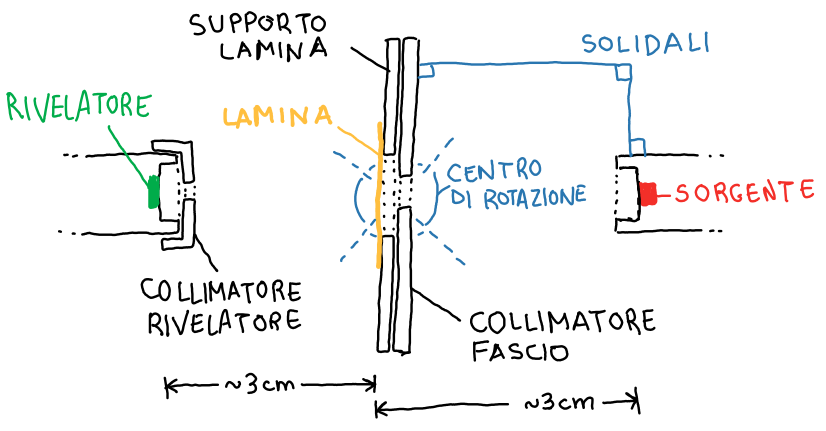
\includegraphics[width=28em]{immagini/schemacamera}
	\caption{\label{fig:schemacamera}
	Schema essenziale dell'apparato di misura.}
\end{figure}

La parte principale del nostro apparato è costituita da una camera a vuoto cilindrica con un diametro interno di  \SI{16.3(1)}{cm} e altezza \SI{8.4(1)}{cm} a cui è collegata la relativa pompa e i vacuometri.
% \marginpar{ha senso scrivere l'errore su ste misure ? (Bob)} % sticazzi

Nel centro è possibile inserire un bersaglio che può essere ruotato solidalmente alla sorgente radioattiva $\alpha$
per variare l'angolo tra il proiettile e il rivelatore fisso, un fotodiodo al silicio (vedi \autoref{fig:schemacamera}).
La scheda dell'esperienza afferma che il rivelatore assorbe completamente le particelle $\alpha$,
permettendo di misurarne l'energia.

I bersagli a nostra disposizione sono lamine metalliche di diversi spessori:
\begin{itemize}
	\item oro: \SI{3}{\micro m}, \SI{5}{\micro m}, \SI{20}{\micro m} ($\times$2);
	\item alluminio: \SI{8}{\micro m} ($\times$2);
	\item acciaio: \SI{10}{\micro m};
	\item oro ``calibrato'': \SI2{\micro m};
	\item alluminio ``calibrato'': \SI8{\micro m}.
\end{itemize}
Le lamine ``calibrate'' sono quelle per le quali ci è garantito il valore dello spessore,
le altre lamine erano intese di prova.
Poiché abbiamo saputo solo alla fine dell'esperimento dell'esistenza di questa distinzione,
tutte le misure sono fatte con le lamine ``non calibrate'',
con le lamine ``calibrate'' abbiamo solo fatto delle misure di controllo.
Assumiamo che le lamine di prova siano chiamate tali solo perché sono state maltrattate
da precedenti studenti e che gli spessori siano in realtà altrettanto precisi\footnotemark.
\footnotetext{Sulla lamina d'oro da \SI{3}{\micro m} c'è scritto \SI{0.2}{\micro m},
ma questa è un'altra storia.}

I nostri proiettili sono le particelle $\alpha$ emesse da una sorgente di \am{}
con attività \SI{330}{kBq} nel 1990 che si riduce a \SI{315}{kBq} nel 2018.
La scheda afferma che la sorgente è chiusa da uno strato di \SI3{\micro m} di metallo,
che gli studenti di un gruppo precedente ci comunicano essere d'oro.
Possiamo scegliere di collimare il fascio incidente con due collimatori in plastica aventi una fessura rettangolare larga \SI{1}{mm} o \SI{5}{mm} ed altezza di \SI{5}{cm}.
La lamina bersaglio è in ogni caso accoppiata a una maschera circolare di diametro \SI{12}{mm}.
Il fotodiodo ha davanti a sé un collimatore rettangolare di dimensioni $2\times 6$\,\si{mm^2} rotabile a piacere,
che però lasceremo sempre in posizione verticale.

\paragraph{Elettronica di misura}

L'energia dei segnali del fotodiodo è misurata con un circuito preamplificatore-amplificatore-ADC.
Il circuito è triggerato da un discriminatore a soglia in tensione sul segnale del fotodiodo.
L'ADC è a 12 bit e fornisce anche il timestamp dell'evento con un round-time di 1.8 ore
e una risoluzione di \SI{0.1}s.
I segnali triggerati vengono anche contati da un modulo contatore.
Usiamo un timer in modalità bistabile per avviare e fermare contemporaneamente
il contatore e il circuito di misura dell'energia; il tempo è misurato dal conteggio \texttt{clock} del contatore. 
